\newcommand{\nom}{Porte conteneur}
\newcommand{\sequence}{03}
\newcommand{\num}{04}
\newcommand{\type}{TD}
\newcommand{\descrip}{Résolution d'un problème en utilisant des méthodes algorithmiques}
\newcommand{\competences}{Alt-C3: Concevoir un algorithme répondant à un problème précisément posé}
\documentclass[10pt,a4paper]{article}
  \usepackage[french]{babel}
  \usepackage[utf8]{inputenc}
  \usepackage[T1]{fontenc}
  \usepackage{xcolor}
  \usepackage[]{graphicx}
  \usepackage{makeidx}
  \usepackage{textcomp}
  \usepackage{amsmath}
  \usepackage{amssymb}
  \usepackage{stmaryrd}
  \usepackage{fancyhdr}
  \usepackage{lettrine}
  \usepackage{calc}
  \usepackage{boxedminipage}
  \usepackage[french,onelanguage, boxruled,linesnumbered]{algorithm2e}
  \usepackage[colorlinks=false,pdftex]{hyperref}
  \usepackage{minted}
  \usepackage{url}
  \usepackage[locale=FR]{siunitx}
  \usepackage{multicol}
  \usepackage{tikz}
  \makeindex

  %\graphicspath{{../Images/}}

%  \renewcommand\listingscaption{Programme}

  %\renewcommand{\thechapter}{\Alph{chapter}}
  \renewcommand{\thesection}{\Roman{section}}
  %\newcommand{\inter}{\vspace{0.5cm}%
  %\noindent }
  %\newcommand{\unite}{\ \textrm}
  \newcommand{\ud}{\mathrm{d}}
  \newcommand{\vect}{\overrightarrow}
  %\newcommand{\ch}{\mathrm{ch}} % cosinus hyperbolique
  %\newcommand{\sh}{\mathrm{sh}} % sinus hyperbolique

  \textwidth 160mm
  \textheight 250mm
  \hoffset=-1.70cm
  \voffset=-1.5cm
  \parindent=0cm

  \pagestyle{fancy}
  \fancyhead[L]{\bfseries {\large PTSI -- Dorian}}
  \fancyhead[C]{\bfseries{{\type} \no \numero}}
  \fancyhead[R]{\bfseries{\large Informatique}}
  \fancyfoot[C]{\thepage}
  \fancyfoot[L]{\footnotesize R. Costadoat, C. Darreye}
  \fancyfoot[R]{\small \today}
  
  \definecolor{bg}{rgb}{0.9,0.9,0.9}
  
  
  % macro Juliette
  
\usepackage{comment}   
\usepackage{amsthm}  
\theoremstyle{definition}
\newtheorem{exercice}{Exercice}
\newtheorem*{rappel}{Rappel}
\newtheorem*{remark}{Remarque}
\newtheorem*{defn}{Définition}
\newtheorem*{ppe}{Propriété}
\newtheorem{solution}{Solution}

\newcounter{num_quest} \setcounter{num_quest}{0}
\newcounter{num_rep} \setcounter{num_rep}{0}
\newcounter{num_cor} \setcounter{num_cor}{0}

\newcommand{\question}[1]{\refstepcounter{num_quest}\par
~\ \\ \parbox[t][][t]{0.15\linewidth}{\textbf{Question \arabic{num_quest}}}\parbox[t][][t]{0.85\linewidth}{#1\label{q\the\value{num_quest}}}\par
~\ \\}

\newcommand{\reponse}[4][1]
{\noindent
\rule{\linewidth}{.5pt}\\
\textbf{Question\ifthenelse{#1>1}{s}{} \multido{}{#1}{%
\refstepcounter{num_rep}\ref{q\the\value{num_rep}} }:} ~\ \\
\ifdef{\public}{#3 ~\ \\ \feuilleDR{#2}}{#4}
}

\newcommand{\cor}
{\refstepcounter{num_cor}
\noindent
\rule{\linewidth}{.5pt}
\textbf{Question \arabic{num_cor}:} \\
}



\begin{document}

\begin{center}
{\Large\bf TP \no {\numero} -- \descrip}
\end{center}

\SetKw{KwFrom}{de} 


\section{R\' esolution d'\' equations du second ordre}
\noindent L'objectif est de r\' esoudre les \' equations de type $(E)\colon ax^2+bx+c=0$ o\` u $a,b$ et $c$ sont des r\' eels, (donc seront des flottants dans vos programmes).

\begin{exercice}
Dans cet exercice, on suppose que $a\neq 0$.\\
\' Ecrire une fonction \verb?solution(a,b,c)? qui renvoie les solutions de $(E)\colon ax^2+bx+c=0$ et pr\' ecise la nature de ses solutions. Par exemple :
\begin{minted}[frame=lines]{python}
>>> solution(2,-6,4)
Deux solutions reelles  x1=1.0 et x2=2.0
>>> solution(4,-4,1)
Une solution double  x=0.5
>>> solution(1,-2,2)
Deux solutions complexes  x1=1+1j et x2=1-1j
\end{minted}
\end{exercice}


\begin{exercice}
Dans cet exercice, $(E)$ n'est pas forc\' ement une \' equation du second degr\' e : $a$ peut \^ etre nul.\\
Ecrire une fonction \verb?solution2? pour prendre en compte tous les cas. (On commencera par construire sur feuille un algorigramme.)\\
Par exemple :
\begin{minted}[frame=lines]{python}
>>> solution2(1,-3,2)
Deux solutions reelles : x1=1.0 et x2=2.0
>>> solution2(0,2,0)
Une solution reelle : x=0.0
>>> solution2(0,0,1)
Pas de solution
>>> solution2(0,0,0)
Une infinite de solutions : tous les reels
\end{minted}
\end{exercice}


\begin{exercice}
\begin{enumerate}
\item R\' esolvez \textbf{\` a la main} l'\' equation suivante : 
\[(E_5)\colon x^2+(1+2^{-50})x+0,25+2^{-51}=0\]
\item R\' esolvez cette \' equation \` a l'aide de la fonction \verb?solution?. Que constatez-vous ? Pourquoi ?
\end{enumerate}
\end{exercice}

\begin{exercice}
\begin{enumerate}
\item R\' esolvez \textbf{\` a la main} les deux \' equations suivantes : 
\[(E_3)\colon x^2+6x+9\qquad (E_4)\colon 0.1x^2+0.6x+0.9=0\]
\item R\' esolvez ces \' equations \` a l'aide de la fonction \verb?solution?. Que constatez-vous ? Pourquoi ?
\end{enumerate}
\end{exercice}


\section{R\' esolution par dichotomie}
\noindent \textbf{ATTENTION :} vous aurez besoin de cet algorithme au TP n°10. Donc, sauvegardez proprement et au bon endroit votre programme.
\subsection{Principe}
\noindent Soit $f$ continue telle que $f(a)$ et $f(b)$ soient de signe contraire. Alors un z\' ero de $f$ est dans $[a,b]$.\\
On construit une suite d'intervalles $[a_n,b_n]$ qui contiennent ce z\' ero. A chaque \' etape :\\
on note $c_n=\dfrac{a_n+b_n}{2}$.\\
- si $f(a_n)$ et $f(c_n)$ sont de signe contraire, alors on pose : $a_{n+1}=a_n$ et $b_{n+1}=c_n$.\\
- sinon, on pose : $a_{n+1}=c_n$ et $b_{n+1}=b_n$.\\
On s'arr\^ ete quand $c_n=\dfrac{a_n+b_n}{2}$ est une approximation \` a $\epsilon$ pr\` es d'une solution, autrement dit quand :
\[b_n-a_n\leqslant 2\epsilon\]

\noindent Avantages : d\` es lors que $f(a)$ et $f(b)$ sont de signe contraire et que $f$ est continue, la m\' ethode converge vers une solution. On peut aussi pr\' evoir \` a l'avance le nombre d'it\' erations n\' ecessaires pour une pr\' ecision choisie.\\
Inconv\' enient : la convergence n'est pas tr\` es rapide compar\' ee \` a d'autres m\' ethodes.

\subsection{Application}

\begin{exercice}
Écrire une fonction \verb?dicho? qui prend comme entr\' ee la fonction $f$ \` a \' etudier, les bornes initiales $a$ et $b$, la pr\' ecision $\epsilon$ et qui renvoie $\dfrac{a_n+b_n}{2}$, approximation d’une solution \` a $\epsilon$ pr\` es.
\end{exercice}



\begin{exercice}
\begin{enumerate}
\item Testez la fonction \verb?dicho? sur $f(x)=x^2-2$ pour obtenir une approximation de $\sqrt{2}$ \` a $\epsilon=0,001$ pr\` es.
\item Si on prend $a=2$ et $b=3$, que renvoie le programme ? Est-ce bien l'approximation d'une solution ? Pourquoi le programme renvoie cette valeur ? 
\item Faites en sorte que votre fonction \verb?dicho? affiche un message d'erreur dans ces cas l\` a.
\end{enumerate}
\end{exercice}


\section{R\' esolution avec des suites r\' ecurrentes}

\subsection{Principe}
\noindent L'objectif est de r\' esoudre une \' equation du type $f(x)=x$.\\
On consid\` ere une suite d\' efinie par r\' ecurrence de la fa\c  con suivante :
\[\left\lbrace\begin{array}{l}
u_0=\text{constante}\\
u_{n+1}=f(u_n)
\end{array}\right.\qquad (*)\]
Dans certains cas favorables, la suite $(u_n)_{n\in\mathbb{N}}$ converge. \` A ce moment l\` a, sa limite est un point fixe de $f$, c'est-\` a-dire une solution de $f(x)=x$.

\subsection{Application}

\begin{exercice}
\' Ecrire une fonction \verb?rec? qui prend comme entr\' ee $f,u_0,n$ et qui renvoie $u_n$, le $n$i\` eme terme de la suite d\' efinie par r\' ecurence en $(*)$.
\end{exercice}

\noindent \begin{minipage}{10cm}
\begin{exercice}\label{racine}
Tester votre fonction \verb?rec? avec $f(x)=\dfrac{1}{2}\left(x+\dfrac{2}{x}\right)$ et $u_0\in\mathbb{R}^*$.\\
On peut montrer que la suite $(u_n)_{n\in\mathbb{N}}$ converge et que les points fixes de $f$ sont : $\sqrt{2}$ et $-\sqrt{2}$. 
\end{exercice}
\end{minipage}
\begin{minipage}{10cm}
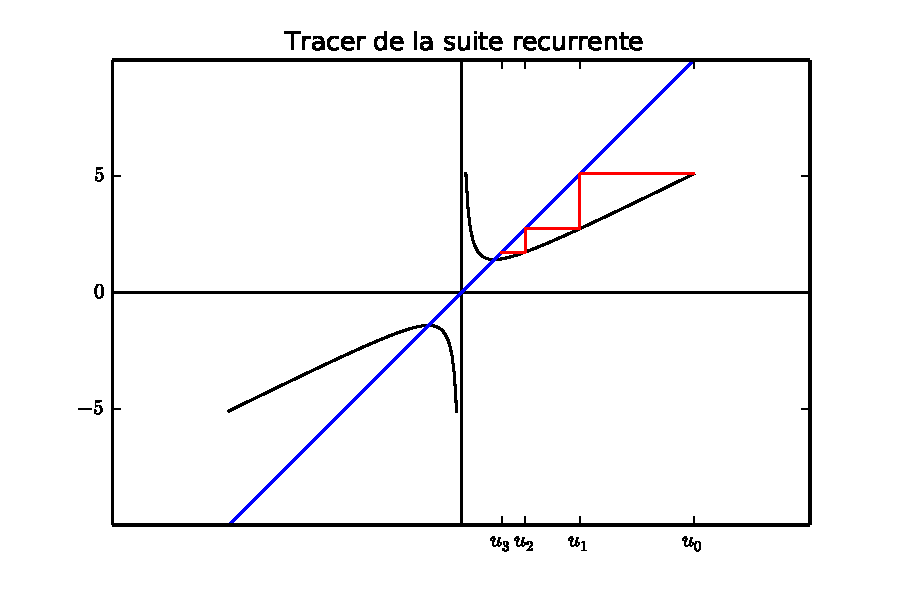
\includegraphics[scale=0.5]{Dessin/TracerSuite.pdf}
\end{minipage}



\begin{exercice}
Avec la fonction \verb?dicho? appliqu\' ee \` a $g(x)=f(x)-x$, on retrouve les solutions de $f(x)=x$.\\
Testez-le avec la fonction $f$ de l'exercice pr\' ec\' edent.\\
Entre \verb?dicho? et \verb?rec?, quel est l'algorithme le plus rapide ? 
\end{exercice}


\newpage


\section{Annexe : les complexes}
\noindent Un complexe se note : \verb?z=1+2j?. \\
\textbf{Attention :} si vous voulez le complexe $z=j$, il faut \' ecrire \verb?z=1j? et non pas \verb?z=j? car Python consid\` ere alors \verb?j? comme une variable et non comme le complexe $j$.\\
Quelques fonctions :\\
\begin{tabular}{llll}
\verb?z.real ? & partie r\' eelle de $z$\\
\verb?z.imag ? & partie imaginiare de $z$\\
\verb?z.conjugate() ? & conjugu\' e de $z$\\
\verb?abs(z) ? & module de $z$
\end{tabular}




\ifdef{\public}{\end{document}}{}

\newpage 

\begin{center}
{\Large\bf Correction TP \no {\numero} -- \descrip}
\end{center}



\begin{solution}~\\
\vspace*{-0.7cm}
\begin{minted}[frame=lines]{python}
from math import sqrt
def solution(a,b,c):
	delta=b**2-4*a*c
	if delta >0:
		x1=(-b+sqrt(delta))/float(2*a)
		x2=(-b-sqrt(delta))/float(2*a)
		return "Deux solutions reelles", x1,x2
	elif delta==0:
		x=-b/float(2*a)
		return "Une solution double" ,x
	else:
		x1=(-b+sqrt(-delta)*1j)/float(2*a)
		x2=(-b-sqrt(-delta)*1j)/float(2*a)
		return "Deux solutions complexes", x1,x2			
		
print solution(2,-6,4)		
\end{minted}
\end{solution}



\begin{solution}
~\\
\vspace*{-0.7cm}
\begin{minted}[linenos,frame=lines]{python}
def solution2(a,b,c):
	if a != 0:
		return(solution(a,b,c))
	else:
		if b!=0:
			return "Une solution reelle" , -c/float(b)
		else :
			if c!=0:
				return "pas de solution"
			else:
				return "Une infinite de solutions : tous les reels."	

print solution(0,0,0)								
\end{minted}
\end{solution}



\begin{solution}
\begin{enumerate}
\item $\Delta=1+2^{-49}+2^{-100}-1-2^{-49}=2^{-100}\neq 0$.\\
On trouve deux solutions r\' eelles distinctes.
\item \verb?solution(1,(1+2**(-50)),0.25+2**(-51))? renvoie une unique solution. En effet, dans la repr\' esentation des nombres, on a vu que Python admet une limite de pr\' ecision pour les flottants. $2^{-100}$ d\' epasse cette limite et Python \' evalue $\Delta$ \` a z\' ero.
\end{enumerate}
\end{solution}




\begin{solution}
\begin{enumerate}
\item Dans les deux cas, on trouve une solution double : $x=-3$
\item \verb?solution(1,6,9)? renvoie l'unique solution \verb?-3?. Mais \verb?solution(0.1,0.6,0.9)? renvoie deux solutions complexes.\\
Dans le premier cas, $\Delta$ est un entier. Python le compare \` a z\' ero sans erreur. Dans le deuxi\` eme cas, $\Delta$ est un flottant qui vaut $\approx -5.10^{-17}$. Le comparer \` a z\' ero n'est plus exact.
\end{enumerate}
\end{solution}



\begin{solution} ~\\
\vspace*{-0.7cm}
\begin{minted}[linenos,frame=lines]{python}
def dicho(f,a,b,eps):               
    while (b-a)>2*eps:
        c=(float(a)+b)/2
        if f(a)*f(c)<0:
            b=c
        else:
            a=c    
    return((a+b)/2)    
\end{minted}
\end{solution}

\newpage

\begin{solution}
 ~\\
\vspace*{-0.7cm}
\begin{enumerate}
\item \begin{minted}[linenos,frame=lines]{python}
def carre(x):
	return(x**2-2)    
\end{minted}
\item Sur $[2,3]$, $f$ ne s'annule pas. Donc dans l'algorithme, on aura toujours $f(a)f(c)>0$, donc \verb?a=c?.\\
Le programme renvoie donc $3-\epsilon$.
\item  \begin{minted}[linenos,frame=lines]{python}
def dicho(f,a,b,eps):               
    if f(a)*f(b)>0:
        return('nous ne savons pas si f s annule entre a et b')
    while (b-a)>2*eps:
        c=(float(a)+b)/2
        if f(a)*f(c)<0:
            b=c
        else:
            a=c    
    return((a+b)/2)
\end{minted}
\end{enumerate}
\end{solution}



\begin{solution}~\\
\vspace*{-0.7cm}
\begin{minted}[linenos,frame=lines]{python}
def rec(f,u,n):
   for i in range(n):
   u=f(u)
   return(u)
\end{minted}
\end{solution}


\begin{solution}
Selon le choix de $u_0\neq 0$, la suite converge vers $\sqrt{2}$ ou $-\sqrt{2}$.
\end{solution}


\begin{solution}
Avec \verb?dicho(g,1,2,0.001)?, on trouve une approximation de $\sqrt{2}$ \` a $0,001$ pr\` es.\\
Pour comparer les deux programmes, on ajoute un compteur \` a la fonction \verb?dicho? pour compter le nombre d'it\' erations effectu\' ees par l'algorithme :
\begin{minted}[linenos,frame=lines]{python}
def dicho(f,a,b,eps):
	compteur=0               
    if f(a)*f(b)>0:
        return('nous ne savons pas si f s annule entre a et b')
    while (b-a)>2*eps:
    	compteur=compteur+1
        c=(float(a)+b)/2
        if f(a)*f(c)<0:
            b=c
        else:
            a=c    
    return((a+b)/2,compteur)
\end{minted}
Par exemple, pour \verb?dicho(g,1,2,0.001)?, on obtient les trois premiers chiffres de $\sqrt{2}$ en 9 it\' erations. \\
Avec \verb?rec(f,1,9)?, on obtient les 12 premiers chiffres de $\sqrt{2}$.\\
La fonction \verb?rec? est donc plus rapide que \verb?dicho?.
\end{solution}




\end{document}























\section{GNA : Reste}


\section{Manipulation de tableaux}
\begin{defn}
Dans la section suivante, nous travaillerons \` a l'aide de tableaux. Importez le module numpy qui permet de nombreuses manipulations.\\
Un tableau sera vu comme une liste de listes. \\
Exemple : $T=[[1,2,3],[-1,4,2],[0,6,5],[12,1,-4]]$.
\end{defn}

\begin{exercice}
\begin{enumerate}
\item Recopier le tableau T en prenant soin d'en faire un tableau numpy. V\' erifier son type.
\item Extraire la premi\` ere ligne de $T$.
\item Extraire le terme \verb?4? de $T$.
\item \' Ecrire un programme qui affiche tous les termes de $T$ :
\begin{verbatim}
1
2
3
-1
\end{verbatim}
etc...
\end{enumerate}
\end{exercice}

\begin{exercice}
\begin{enumerate}
\item Que renvoie \verb?T+T?, \verb?3*T? ? Qu'aurions nous obtenu si $T$ \' etait une liste ?\\
Notez que l'addition et la multiplication externe sur des tableaux numpy sont les op\' erations matricielles vues en cours de maths.
\item Pour concat\' ener deux tableaux numpy \` a deux dimensions, on peut utiliser la fonction numpy \verb?concatenate? qui prend comme argument, les deux tableaux ou parties de tableaux, et une option \verb?axis?.\\
Testez la fonction sur les tableaux suivants. Que fait l'option \verb?axis? ?
\begin{verbatim}
A=np.array([[1,2,3],[4,5,6]])
B=np.array([[7,8,9],[10,11,12]])
C=np.concatenate((A,B),axis=0)
D=np.concatenate((A,B),axis=1)
\end{verbatim}
\end{enumerate}
\end{exercice}

\begin{exercice}
\' Ecrire une fonction \verb?taille? qui renvoie la taille d'un tableau.
\end{exercice}


\begin{exercice}
\begin{enumerate}
\item \' Ecrire une fonction \verb?maximum? qui renvoie le maximum d'un tableau :
\begin{verbatim}
>>>maximum(T)
12
\end{verbatim}
\item \' Ecrire une fonction \verb?positionmax? qui renvoie la position du maximum d'un tableau :
\begin{verbatim}
>>>positionmax(T)
(3,0)
\end{verbatim}
\end{enumerate}
\end{exercice}


\begin{exercice}[Pour aller plus loin : \` a faire si vous \^ etes en avance ou \` a la fin du TD]~\\
Que se passe-t-il si le maximum apparait plusieurs fois dans le tableau ? \\
Modifier la fonction pour que toutes les positions apparaissent. \\
Testez la fonction sur $T1=[[1,1],[0,1]]$
\end{exercice}


\begin{exercice}
\begin{enumerate}
\item Une fonction \verb?max? existe. Testez-la sur nos exemples.
\item Pour trouver la position du maximum, on peut utiliser la fonction numpy \verb?where? :\\
\verb?np.where? (condition) renvoie les positions du tableau o\` u la condition est v\' erifi\' ee. \\
Dans $T$, quelles sont les valeurs sup\' erieures strictes \` a 4 ? En quelles positions sont-elles ?
\item Testez les commandes suivantes et v\' erifiez les r\' esultats :\\
\verb?np.where(T>4)?, \verb?np.where(T=1)? \footnote{Pourquoi cela renvoie-t-il un message d'erreur ? Corrigez}, \verb?np.where(T<-100)?
\item \' Ecrire une commande qui permet d'avoir les positions du maximum de $T$.
\end{enumerate}
\end{exercice}


